\documentclass{beamer}
\usepackage[english]{babel}
\usepackage[latin1]{inputenc}
\usepackage[T1]{fontenc}
\usepackage{amssymb}
\usepackage{amsmath}
\usepackage{booktabs}
\usepackage{verbatim}
\usepackage{caption}
\usepackage{float}
\usepackage{csquotes}
\usepackage{sansmathaccent}
\usepackage{subfigure}
\usepackage{multicol}
\pdfmapfile{+sansmathaccent.map}
\def \ourFigPath {../../} 
\def \ourTablePath {../../Tables/} 

\setbeamersize{text margin left=5mm,text margin right=12mm} 
%
\font\reali=msbm10 at 12pt
% subsets of real numbers
\newcommand{\numberset}{\mathbb}
\newcommand{\real}{\hbox{\reali R}}
\newcommand{\N}{\numberset{N}}
\newcommand{\realp}{\hbox{\reali R}_{\scriptscriptstyle +}}
\newcommand{\realpp}{\hbox{\reali R}_{\scriptscriptstyle ++}}
\newcommand{\virgolette}[1]{``#1''}
%

\author[Brianti, Gati]{Marco Brianti and Laura Gati}

\institute[Boston College]{Boston College}


\title{IT Spillovers in TFP }

\date{\today}

\usetheme{Warsaw}


\begin{document}


\begin{frame}

\maketitle


\end{frame}

%%%%%%% Slide %%%%%%
\begin{frame}
\frametitle{Household}

$$
\max_{C_t, \ H_t, \ K_t^C, \ K_t^I} \sum_{j=0}^{\infty} \beta^j \bigg[ \log C_t -  \frac{1}{2} H_t^2 \bigg]
$$

\

subject to

\


$$
Y^C_t = C_t + I^C_t \ \ \text{and} \ \ Y_t^I = I^I_t;
$$


$$
K^C_{t+1} = (1 - \delta^C)K^C_t + I^C_t \ \ \text{and} \ \ K^I_{t+1} = (1 - \delta^I)K^I_t + I^I_t;
$$


$$
C_t + K^C_{t+1} + P_t K^I_{t+1} = Y^C_t + P_t Y^I_t + (1 - \delta^C)K^C_t + (1 - \delta^I)P_t K^I_t
$$


\end{frame}
%%%%%%%%%%%%%%%%%

%%%%%%% Slide %%%%%%
\begin{frame}
\frametitle{Production Function}

$$
Y^C_t = S_t^C \  N_t \ (K^I_t)^{\gamma} \ \ \  (H_{1,t})^{1-a-b} \ \ \  (K_{1,t}^C)^{a} \ \ \ (K_{1,t}^I)^{b}
$$
$$
Y^I_t = S_t^I \  N_t \ (K^I_t)^{\gamma} \ \ \  (H_{2,t})^{1-a-b} \ \ \  (K_{2,t}^C)^{a} \ \ \ (K_{2,t}^I)^{b}
$$

\


where

$$
Y^C_t = C_t + I^C_t \ \ \text{and} \ \ Y_t^I = I^I_t;
$$
$$
K^C_{t+1} = (1 - \delta^C)K^C_t + I^C_t \ \ \text{and} \ \ K^I_{t+1} = (1 - \delta^I)K^I_t + I^I_t;
$$

and


$$
H_{1,t} + H_{2,t} = H_t, 
$$
$$
K_{1,t}^C + K_{2,t}^C = K_t^C, 
$$
$$
K_{1,t}^I + K_{2,t}^I = K_t^I
$$





\end{frame}
%%%%%%%%%%%%%%%%%


%%%%%%% Slide %%%%%%
\begin{frame}
\frametitle{Effect on TFP}

\begin{center}
	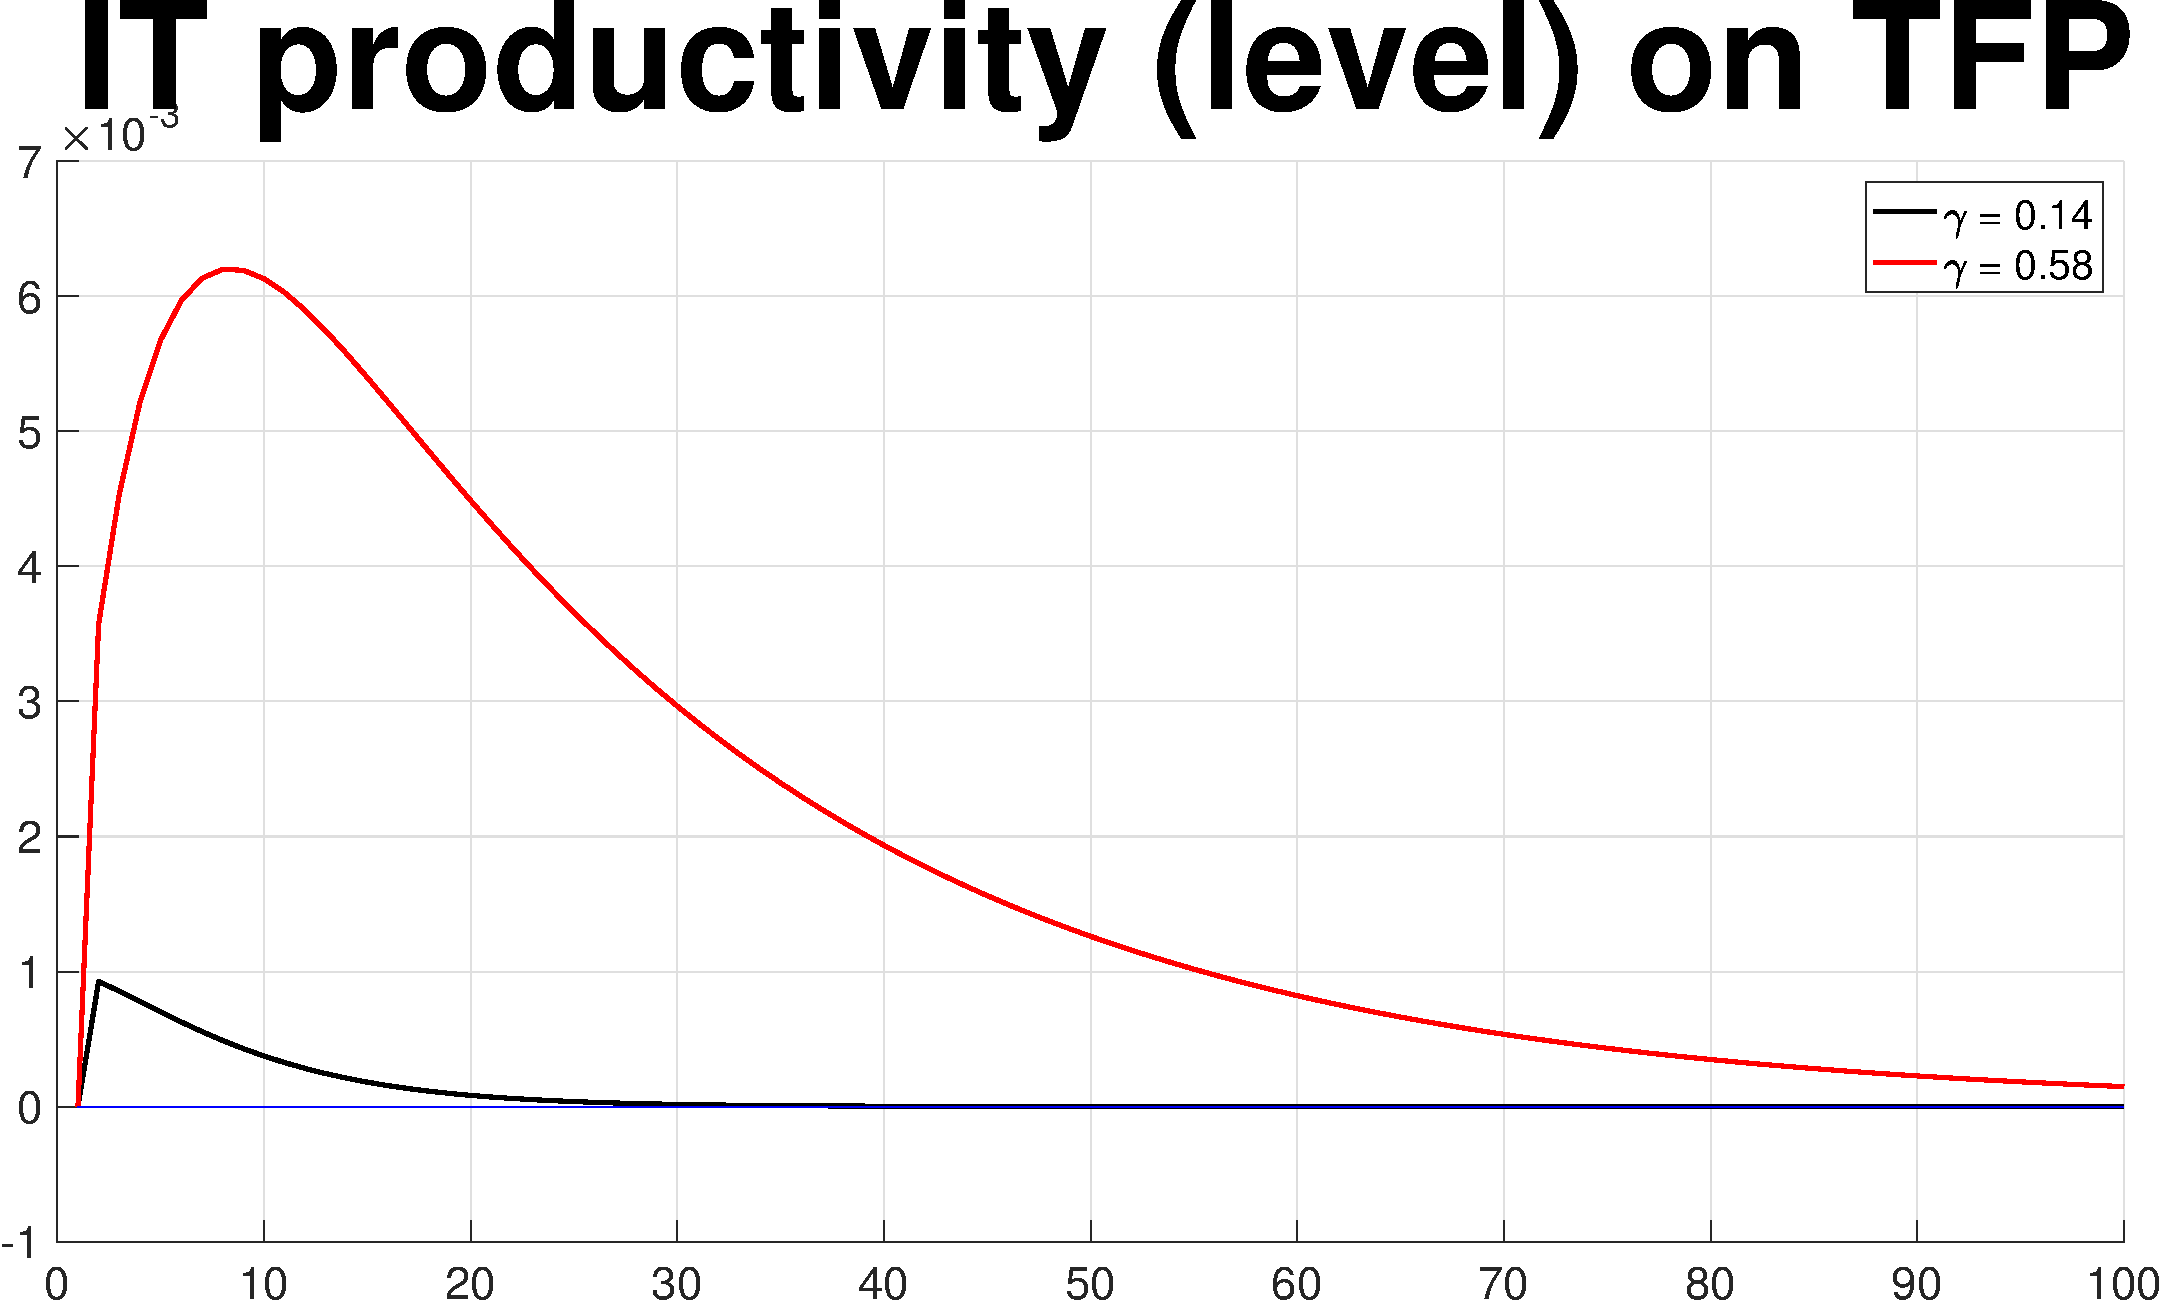
\includegraphics[scale=0.3]{\ourFigPath Figures/fig_IT_productivity_(level)_on_TFP_Varying_gamma}
\end{center}


\end{frame}
%%%%%%%%%%%%%%%%%


%%%%%%% Slide %%%%%%
\begin{frame}
\frametitle{Empirical IRF}

\begin{center}
	\includegraphics[scale=0.15]{\ourFigPath Figures/fig_IT_shock_on_TFP_empirical}
		\includegraphics[scale=0.15]{\ourFigPath Figures/fig_IT_shock_on_Real_IT_Investment_empirical}
\end{center}


\end{frame}
%%%%%%%%%%%%%%%%%


%%%%%%% Slide %%%%%%
\begin{frame}
\frametitle{Empirical IRF}

\begin{center}
	\includegraphics[scale=0.15]{\ourFigPath Figures/fig_IT_shock_on_Real_GDP_empirical}
	\includegraphics[scale=0.15]{\ourFigPath Figures/fig_IT_shock_on_Real_Consumption_empirical}
\end{center}



\end{frame}
%%%%%%%%%%%%%%%%%


%%%%%%% Slide %%%%%%
\begin{frame}
\frametitle{Empirical IRF}

\begin{center}
	\includegraphics[scale=0.15]{\ourFigPath Figures/fig_IT_shock_on_Hours_per_Person_empirical}
	\includegraphics[scale=0.15]{\ourFigPath Figures/fig_IT_shock_on_Relative_Price_empirical}
\end{center}

\end{frame}
%%%%%%%%%%%%%%%%%


\end{document}
